\documentclass[11pt]{article}

% Packages
\usepackage[margin=1in, top=0.7in]{geometry}
\usepackage{amsmath,amssymb,amsfonts}
\usepackage{graphicx}
\graphicspath{{./}{../}}
\usepackage{hyperref}
\usepackage{algorithm}
\usepackage{algpseudocode}
\usepackage{booktabs}
\usepackage{longtable}
\usepackage{multirow}

% Document info
\title{Assignment 2 Report\\
    CS-726: Advanced Machine Learning}
\author{Deeptanshu Malu \quad Deevyanshu Malu \quad Neel Rambhia}
\date{}

\begin{document}

\maketitle

\section{Denoising Diffusion Probabilistic Models}

\subsection{Architecture}

The implemented Denoising Diffusion Probabilistic Model (DDPM) architecture consists of several key components:

\subsubsection{Time Embedding}
We use sinusoidal position embeddings to encode timestep information:
\begin{itemize}
    \item The \texttt{SinusoidalPositionEmbeddings} module transforms scalar timesteps into 16 dimensional embeddings
    \item This creates a unique representation for each timestep that preserves the notion of time progression
    \item The embedding uses a combination of sine and cosine functions at different frequencies, allowing the model to distinguish between timesteps
\end{itemize}

\subsubsection{Network Architecture}
The model consists of:
\begin{itemize}
    \item An input linear layer that maps the concatenation of data and time embeddings to a hidden dimension (128 units)
    \item A series of 5 \texttt{DiffusionBlocks}, each containing a linear layer of 128 units followed by a ReLU activation
    \item An output linear layer that maps back to the data dimensionality
\end{itemize}

Rather than using convolutional layers as in image-based diffusion models, we use fully connected layers which is appropriate for dataset without temporal or spatial structure. The time embedding ensures the model can adapt its behavior based on the specific noise level at each timestep.

\subsection{Results}

For NLL caluclation, the temperature is set to 0.1.
For EMD calculation, the number of subsamples is set to 250 and the number of iterations is set to 5.

For all training runs, the hyperparameters used are as follows:
\begin{itemize}
    \item \textbf{Epochs}: 100
    \item \textbf{Batch Size}: 64
    \item \textbf{Learning Rate}: 1e-3
\end{itemize}

\subsubsection{Varying Timesteps}
Here, lbeta = 0.0001 and ubeta = 0.02.

\begin{longtable}{|l|l|c|c|c|c|c|c|}
    \hline
    \textbf{Dataset} & \textbf{Metric} & \multicolumn{6}{c|}{\textbf{Timesteps}} \\
    \cline{3-8}
    & & \textbf{10} & \textbf{50} & \textbf{100} & \textbf{150} & \textbf{200} & \textbf{500} \\
    \hline
    \multirow{2}{*}{Moons} & EMD & 39.99 & 28.95 & \textbf{27.40} & 29.64 & 30.55 & 44.90 \\
    \cline{2-8}
    & NLL & 1.02 & 0.96 & 0.94 & \textbf{0.93} & 0.94 & 0.95 \\
    \hline
    \multirow{2}{*}{Circles} & EMD & 34.60 & \textbf{31.48} & 33.24 & 34.41 & 38.62 & 42.04 \\
    \cline{2-8}
    & NLL & 1.05 & 0.99 & 1.00 & \textbf{0.98} & 1.01 & 1.03 \\
    \hline
    \multirow{2}{*}{Blobs} & EMD & 88.78 & 43.69 & 20.08 & 18.36 & \textbf{17.17} & 19.83 \\
    \cline{2-8}
    & NLL & 0.34 & 0.12 & 0.04 & 0.03 & \textbf{0.01} & 0.04 \\
    \hline
    \multirow{2}{*}{Manycircles} & EMD & 33.65 & \textbf{26.41} & 27.77 & 27.98 & 30.98 & 30.34 \\
    \cline{2-8}
    & NLL & 0.66 & \textbf{0.54} & \textbf{0.54} & \textbf{0.54} & \textbf{0.54} & 0.58 \\
    \hline
    \multirow{2}{*}{Helix} & EMD & 56.00 & 59.33 & 57.15 & \textbf{56.13} & 58.87 & 60.49 \\
    \cline{2-8}
    & NLL & 1.55 & 1.53 & 1.52 & 1.52 & 1.53 & \textbf{1.51} \\
    \hline
\end{longtable}

\begin{figure}[H]
    \centering
    \begin{tabular}{ccc}
        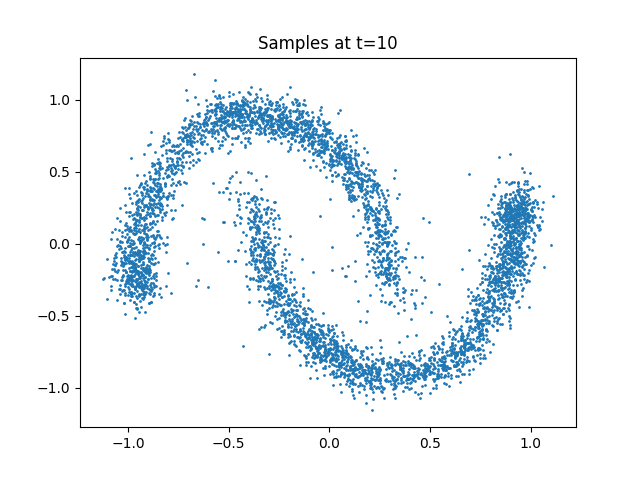
\includegraphics[width=0.3\textwidth]{exps/ddpm_2_10_0.0001_0.02_moons/samples_10.png} &
        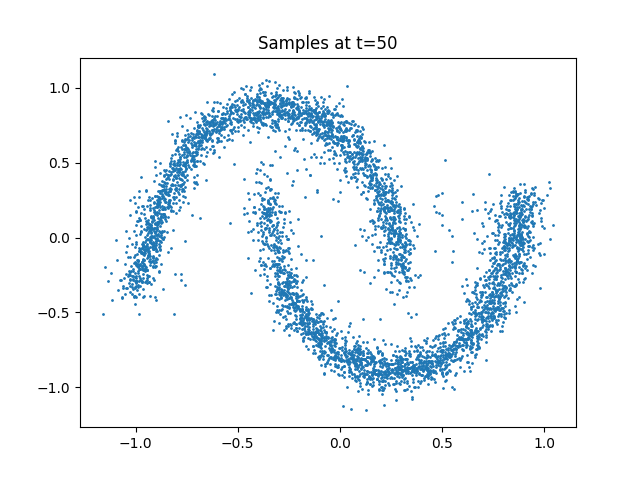
\includegraphics[width=0.3\textwidth]{exps/ddpm_2_50_0.0001_0.02_moons/samples_50.png} &
        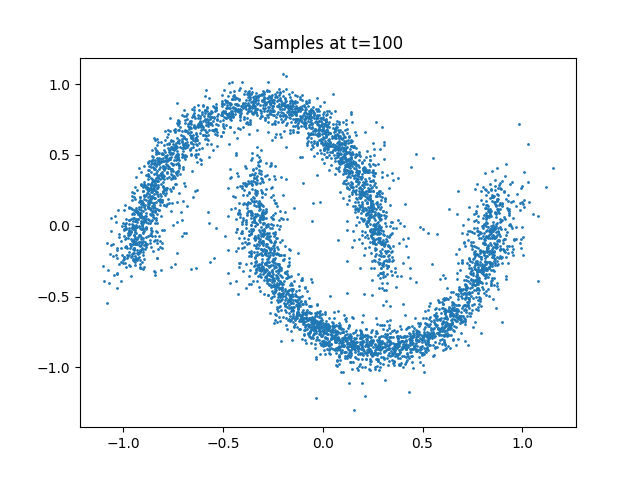
\includegraphics[width=0.3\textwidth]{exps/ddpm_2_100_0.0001_0.02_moons/samples_100.png} \\
        t=10 & t=50 & t=100 \\[0.5em]
        
        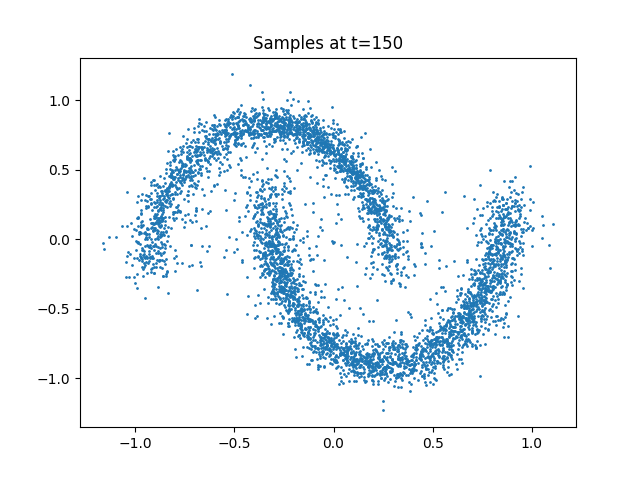
\includegraphics[width=0.3\textwidth]{exps/ddpm_2_150_0.0001_0.02_moons/samples_150.png} &
        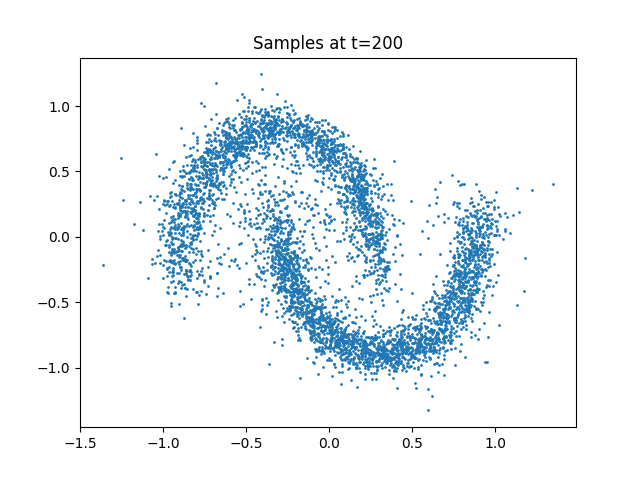
\includegraphics[width=0.3\textwidth]{exps/ddpm_2_200_0.0001_0.02_moons/samples_200.png} &
        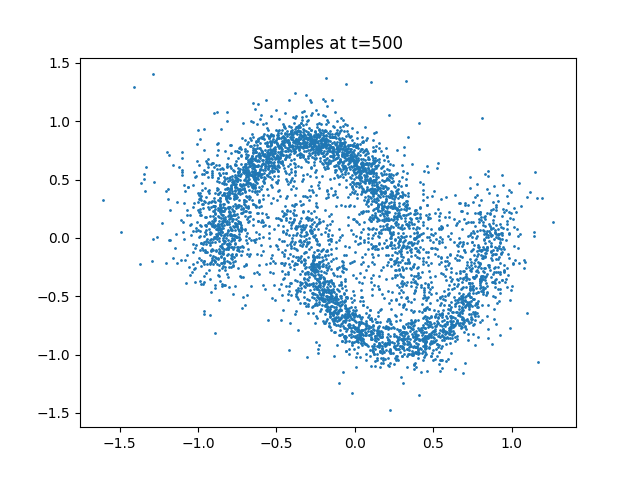
\includegraphics[width=0.3\textwidth]{exps/ddpm_2_500_0.0001_0.02_moons/samples_500.png} \\
        t=150 & t=200 & t=500 \\
    \end{tabular}
    \caption{Samples generated by DDPM with \textbf{varying timesteps} for the Moons dataset.}
    \label{fig:timesteps_moons}
\end{figure}

\begin{figure}[H]
    \centering
    \begin{tabular}{ccc}
        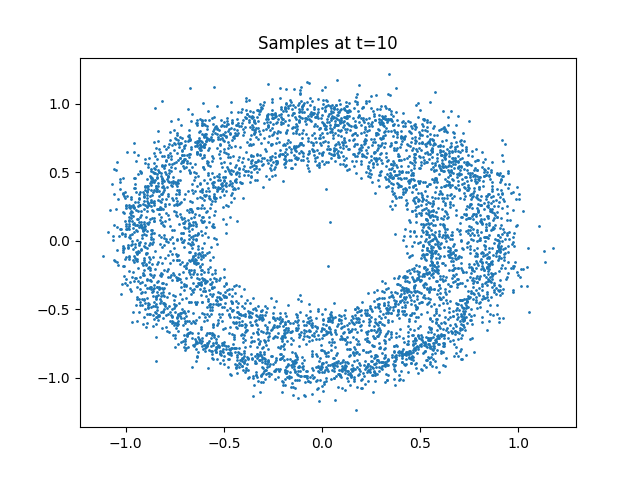
\includegraphics[width=0.3\textwidth]{exps/ddpm_2_10_0.0001_0.02_circles/samples_10.png} &
        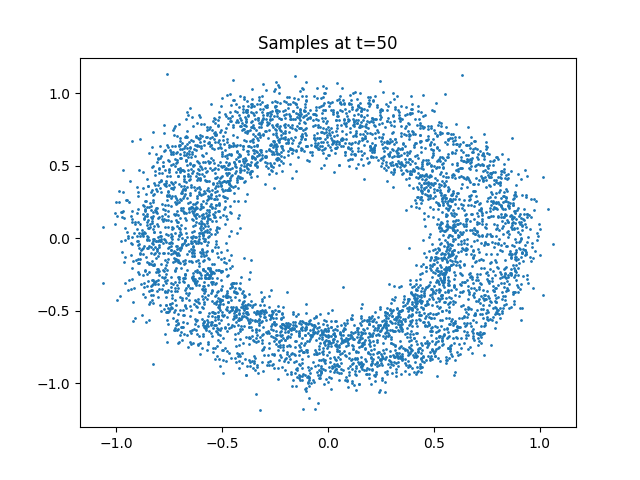
\includegraphics[width=0.3\textwidth]{exps/ddpm_2_50_0.0001_0.02_circles/samples_50.png} &
        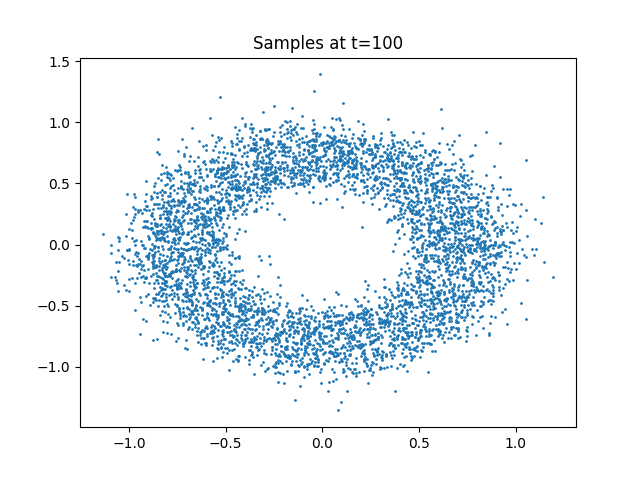
\includegraphics[width=0.3\textwidth]{exps/ddpm_2_100_0.0001_0.02_circles/samples_100.png} \\
        t=10 & t=50 & t=100 \\[0.5em]
        
        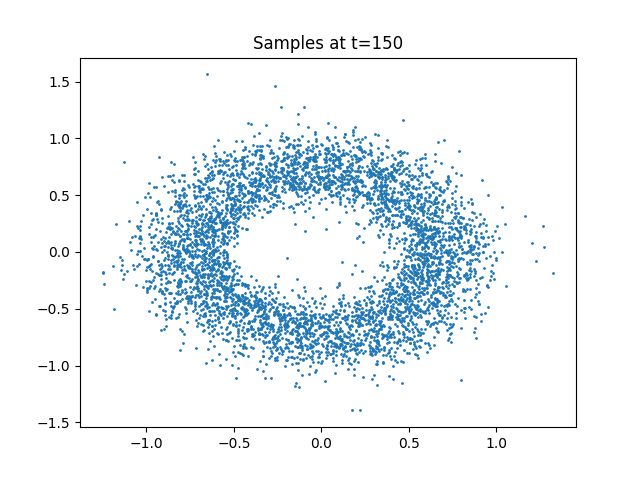
\includegraphics[width=0.3\textwidth]{exps/ddpm_2_150_0.0001_0.02_circles/samples_150.png} &
        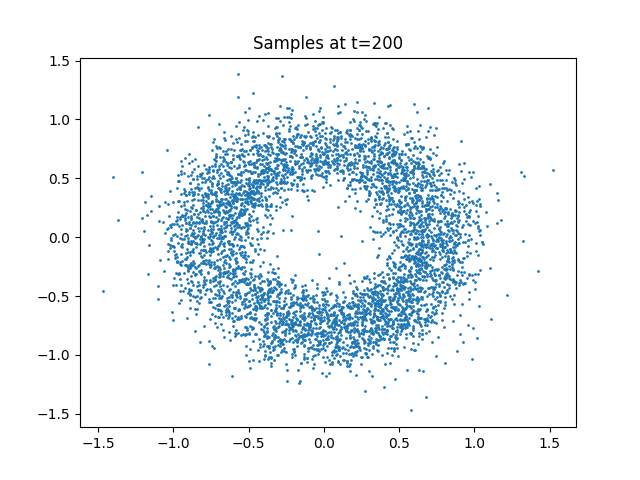
\includegraphics[width=0.3\textwidth]{exps/ddpm_2_200_0.0001_0.02_circles/samples_200.png} &
        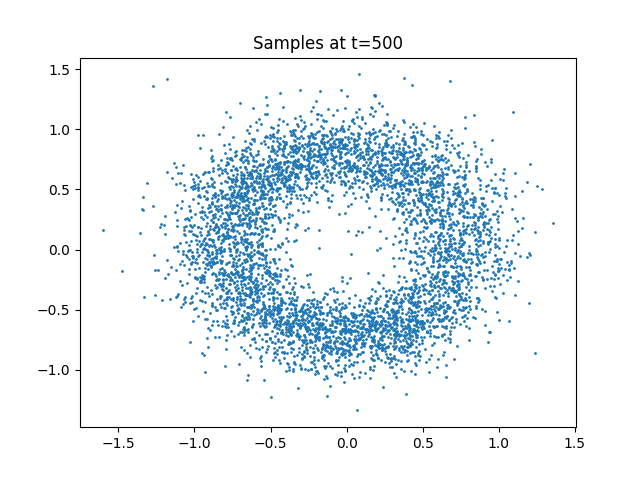
\includegraphics[width=0.3\textwidth]{exps/ddpm_2_500_0.0001_0.02_circles/samples_500.png} \\
        t=150 & t=200 & t=500 \\
    \end{tabular}
    \caption{Samples generated by DDPM with \textbf{varying timesteps} for the Circles dataset.}
    \label{fig:timesteps_circles}
\end{figure}

\begin{figure}[H]
    \centering
    \begin{tabular}{ccc}
        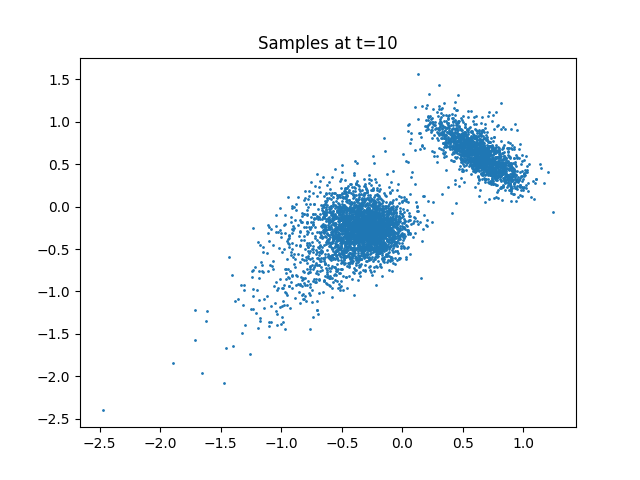
\includegraphics[width=0.3\textwidth]{exps/ddpm_2_10_0.0001_0.02_blobs/samples_10.png} &
        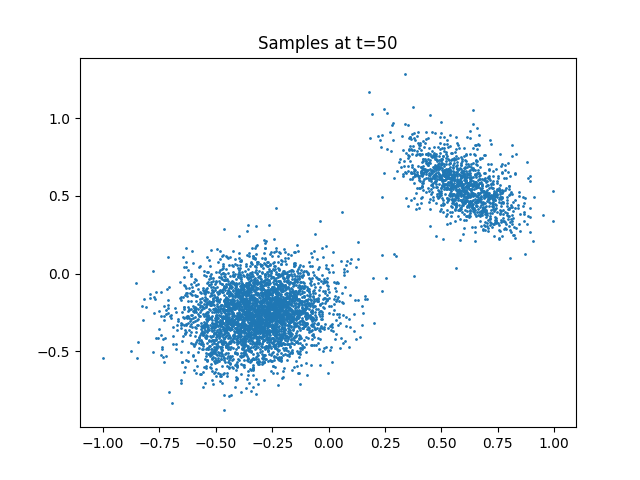
\includegraphics[width=0.3\textwidth]{exps/ddpm_2_50_0.0001_0.02_blobs/samples_50.png} &
        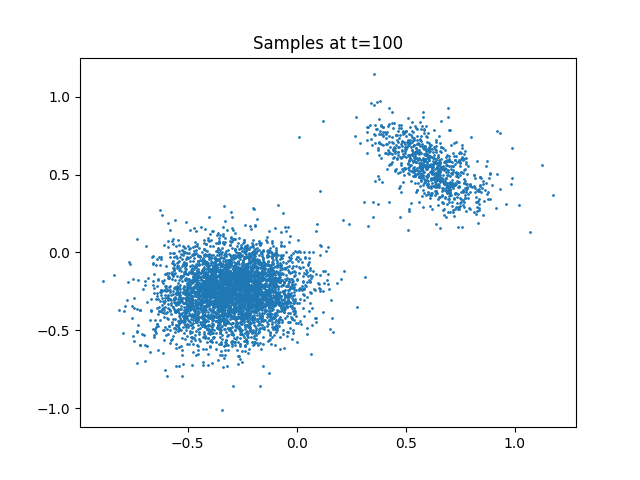
\includegraphics[width=0.3\textwidth]{exps/ddpm_2_100_0.0001_0.02_blobs/samples_100.png} \\
        t=10 & t=50 & t=100 \\[0.5em]
        
        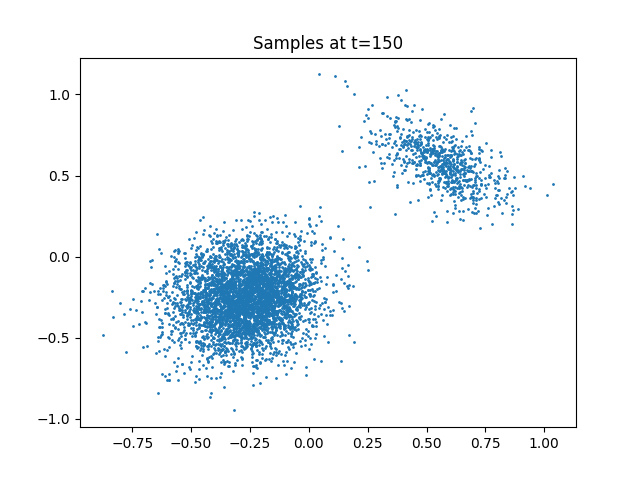
\includegraphics[width=0.3\textwidth]{exps/ddpm_2_150_0.0001_0.02_blobs/samples_150.png} &
        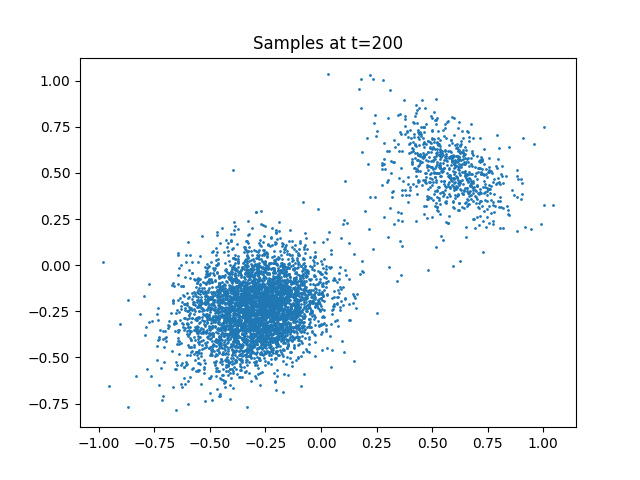
\includegraphics[width=0.3\textwidth]{exps/ddpm_2_200_0.0001_0.02_blobs/samples_200.png} &
        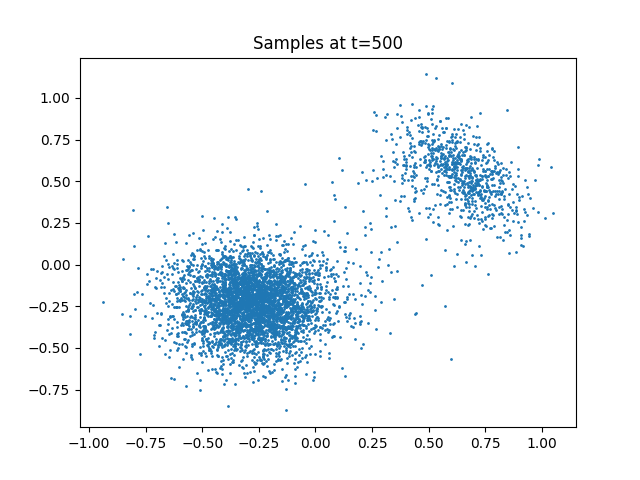
\includegraphics[width=0.3\textwidth]{exps/ddpm_2_500_0.0001_0.02_blobs/samples_500.png} \\
        t=150 & t=200 & t=500 \\
    \end{tabular}
    \caption{Samples generated by DDPM with \textbf{varying timesteps} for the Blobs dataset.}
    \label{fig:timesteps_blobs}
\end{figure}

\begin{figure}[H]
    \centering
    \begin{tabular}{ccc}
        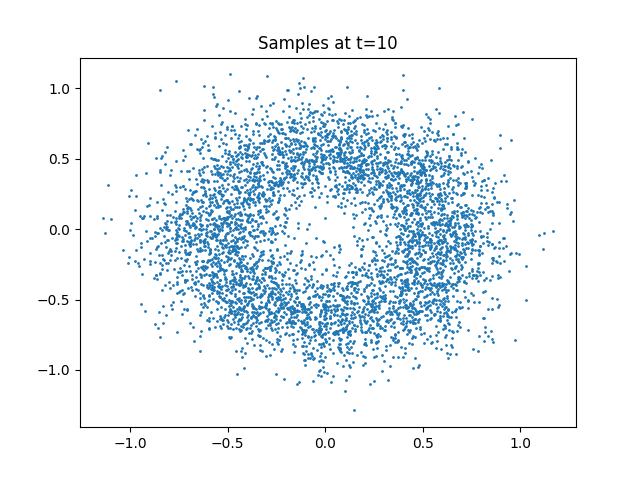
\includegraphics[width=0.3\textwidth]{exps/ddpm_2_10_0.0001_0.02_manycircles/samples_10.png} &
        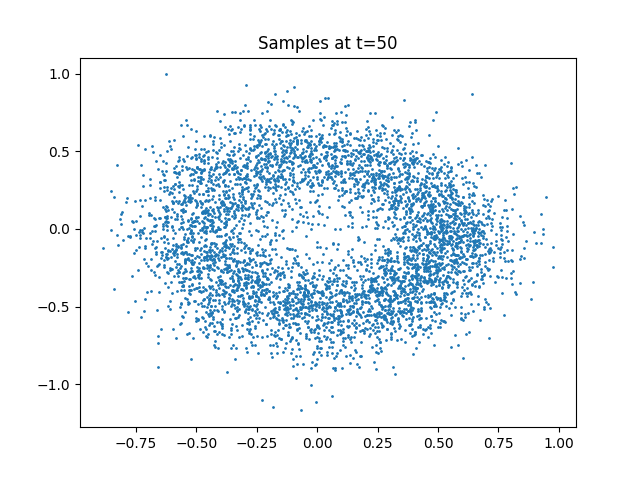
\includegraphics[width=0.3\textwidth]{exps/ddpm_2_50_0.0001_0.02_manycircles/samples_50.png} &
        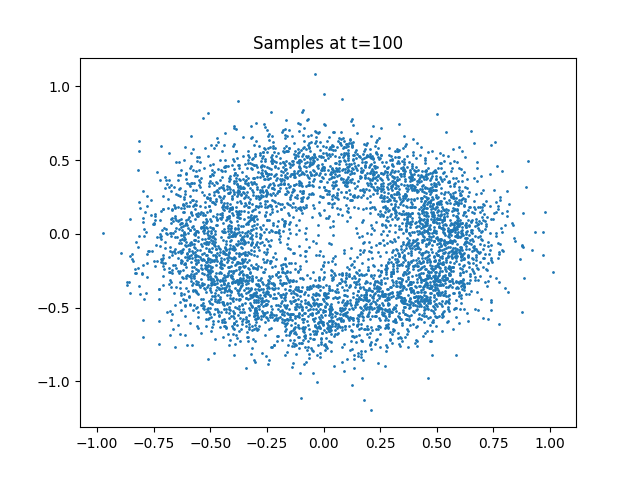
\includegraphics[width=0.3\textwidth]{exps/ddpm_2_100_0.0001_0.02_manycircles/samples_100.png} \\
        t=10 & t=50 & t=100 \\[0.5em]
        
        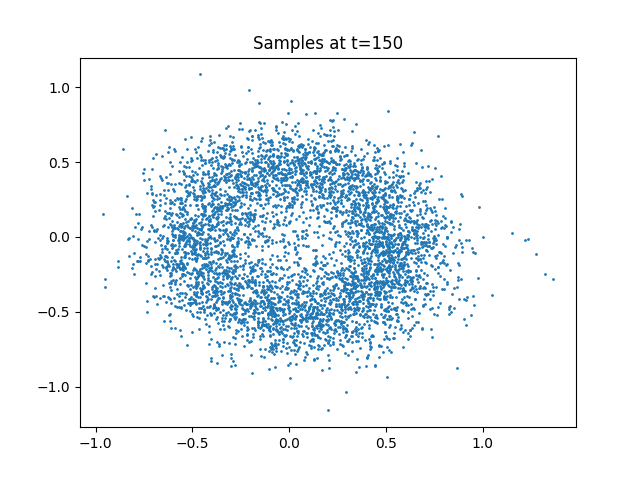
\includegraphics[width=0.3\textwidth]{exps/ddpm_2_150_0.0001_0.02_manycircles/samples_150.png} &
        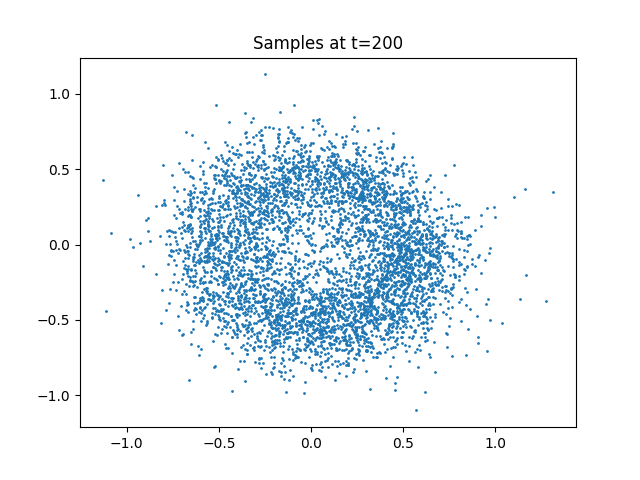
\includegraphics[width=0.3\textwidth]{exps/ddpm_2_200_0.0001_0.02_manycircles/samples_200.png} &
        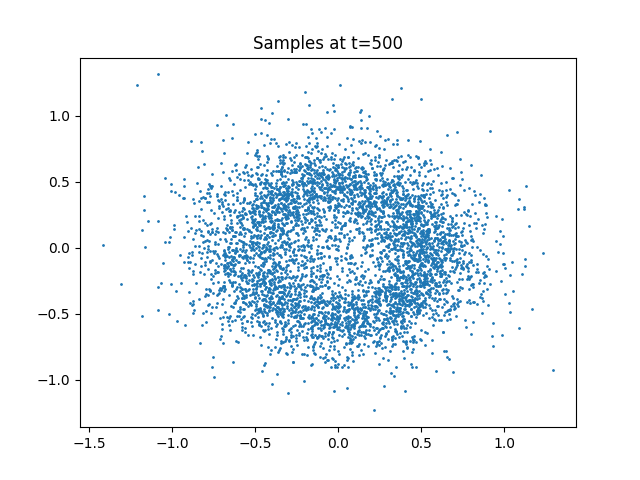
\includegraphics[width=0.3\textwidth]{exps/ddpm_2_500_0.0001_0.02_manycircles/samples_500.png} \\
        t=150 & t=200 & t=500 \\
    \end{tabular}
    \caption{Samples generated by DDPM with \textbf{varying timesteps} for the Manycircles dataset.}
    \label{fig:timesteps_manycircles}
\end{figure}

\begin{figure}[H]
    \centering
    \begin{tabular}{ccc}
        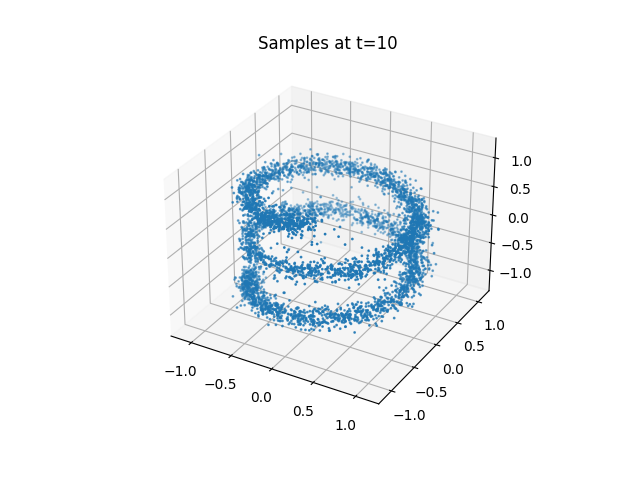
\includegraphics[width=0.3\textwidth]{exps/ddpm_3_10_0.0001_0.02_helix/samples_10.png} &
        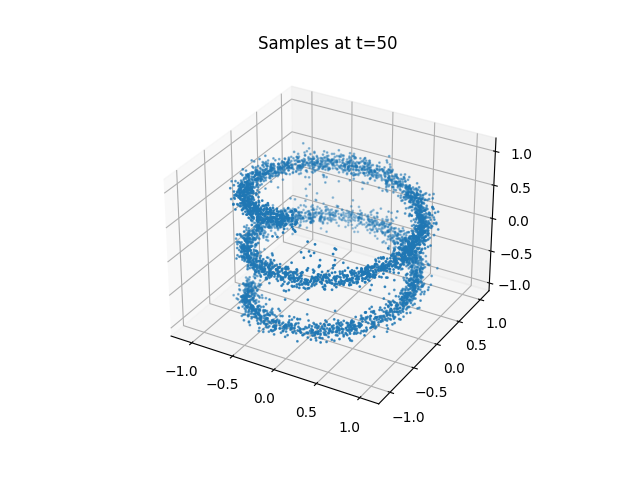
\includegraphics[width=0.3\textwidth]{exps/ddpm_3_50_0.0001_0.02_helix/samples_50.png} &
        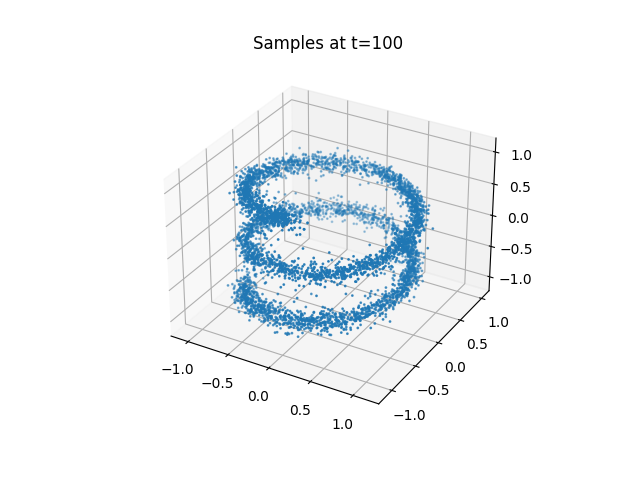
\includegraphics[width=0.3\textwidth]{exps/ddpm_3_100_0.0001_0.02_helix/samples_100.png} \\
        t=10 & t=50 & t=100 \\[0.5em]
        
        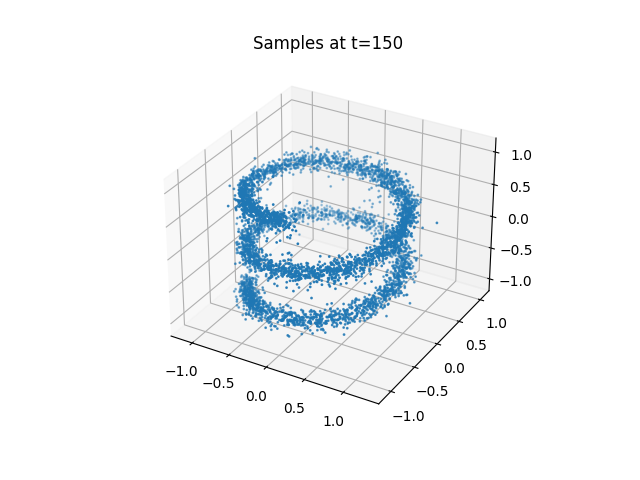
\includegraphics[width=0.3\textwidth]{exps/ddpm_3_150_0.0001_0.02_helix/samples_150.png} &
        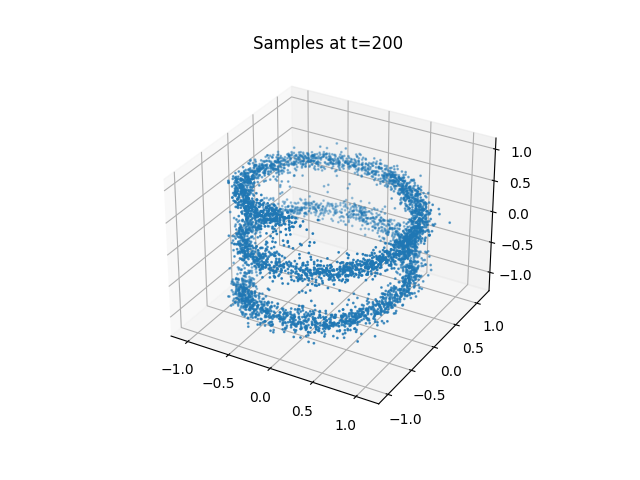
\includegraphics[width=0.3\textwidth]{exps/ddpm_3_200_0.0001_0.02_helix/samples_200.png} &
        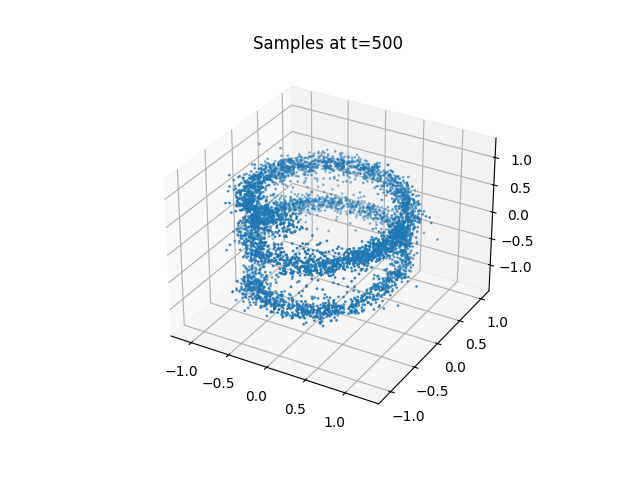
\includegraphics[width=0.3\textwidth]{exps/ddpm_3_500_0.0001_0.02_helix/samples_500.png} \\
        t=150 & t=200 & t=500 \\
    \end{tabular}
    \caption{Samples generated by DDPM with \textbf{varying timesteps} for the Helix dataset.}
    \label{fig:timesteps_helix}
\end{figure}

\subsubsection{Varying Beta Schedule}
Here, timesteps = 200.

\begin{longtable}{|l|l|c|c|c|c|c|c|}
    \hline
     \textbf{Dataset} & \textbf{Metric} & \multicolumn{6}{c|}{\textbf{Beta Schedule (lbeta→ubeta)}} \\
     \cline{3-8}
     & & \textbf{1e-4→0.02} & \textbf{1e-3→0.2} & \textbf{1e-5→0.002} & \textbf{1e-5→0.02} & \textbf{1e-4→0.2} & \textbf{1e-5→0.2} \\
    \hline
        \multirow{2}{*}{Moons} & EMD & 30.55 & 35.57 & 34.76 & \textbf{30.48} & 33.48 & 33.62 \\
        \cline{2-8}
        & NLL & 0.94 & \textbf{0.93} & 0.98 & 0.95 & 0.95 & 0.94 \\
        \hline
        \multirow{2}{*}{Circles} & EMD & 38.62 & 38.03 & \textbf{33.03} & 38.36 & 36.52 & 37.45 \\
        \cline{2-8}
        & NLL & 1.01 & \textbf{1.00} & 1.02 & \textbf{1.00} & 1.01 & 1.01 \\
        \hline
        \multirow{2}{*}{Blobs} & EMD & \textbf{17.17} & 20.35 & 62.98 & \textbf{17.17} & 19.59 & 19.62 \\
        \cline{2-8}
        & NLL & 0.01 & 0.02 & 0.20 & 0.01 & 0.01 & \textbf{0.00} \\
        \hline
        \multirow{2}{*}{Manycircles} & EMD & 30.98 & 28.75 & \textbf{26.55} & 31.82 & 29.40 & 29.92 \\
        \cline{2-8}
        & NLL & 0.54 & \textbf{0.52} & 0.58 & 0.53 & 0.53 & 0.54 \\
        \hline
        \multirow{2}{*}{Helix} & EMD & 58.87 & \textbf{56.25} & 57.31 & 58.29 & 57.34 & 58.72 \\
        \cline{2-8}
        & NLL & 1.53 & \textbf{1.52} & 1.54 & 1.53 & 1.53 & 1.52 \\
        \hline
    \end{longtable}

    \begin{figure}[H]
        \centering
        \begin{tabular}{ccc}
            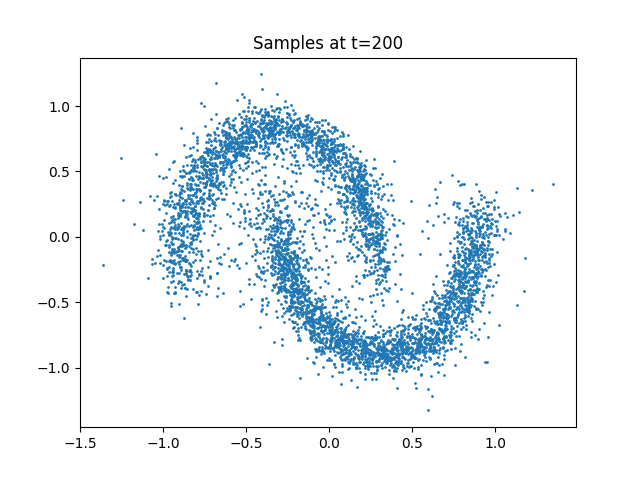
\includegraphics[width=0.3\textwidth]{exps/ddpm_2_200_0.0001_0.02_moons/samples_200.png} &
            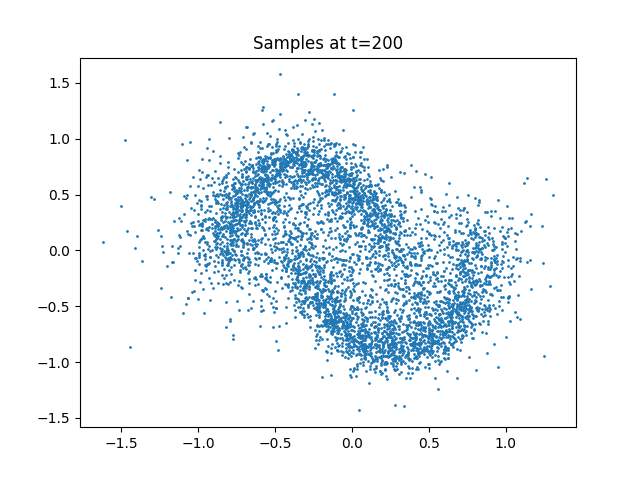
\includegraphics[width=0.3\textwidth]{exps/ddpm_2_200_0.001_0.2_moons/samples_200.png} &
            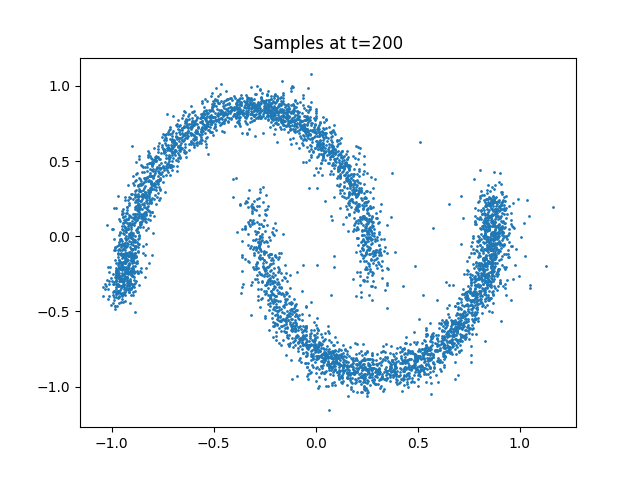
\includegraphics[width=0.3\textwidth]{exps/ddpm_2_200_1e-05_0.002_moons/samples_200.png} \\
            $\beta=1\text{e-}4\to0.02$ & $\beta=1\text{e-}3\to0.2$ & $\beta=1\text{e-}5\to0.002$ \\[0.5em]
            
            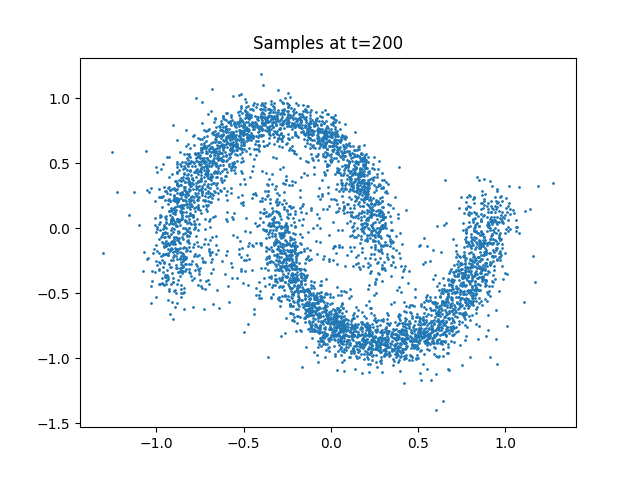
\includegraphics[width=0.3\textwidth]{exps/ddpm_2_200_1e-05_0.02_moons/samples_200.png} &
            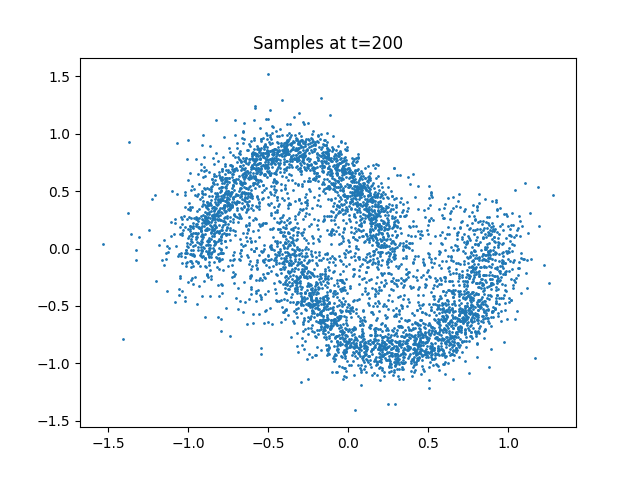
\includegraphics[width=0.3\textwidth]{exps/ddpm_2_200_0.0001_0.2_moons/samples_200.png} &
            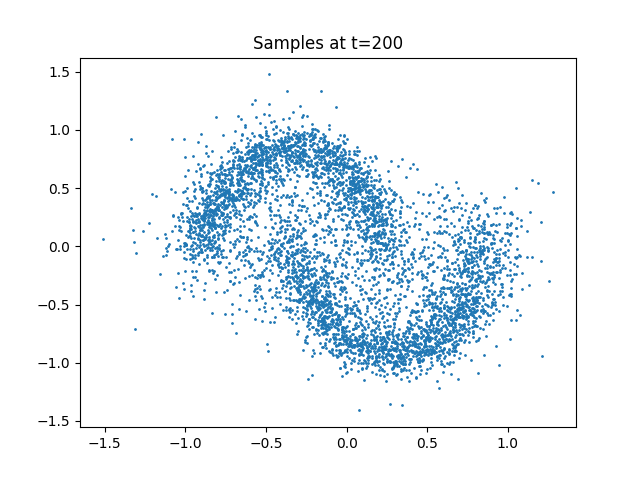
\includegraphics[width=0.3\textwidth]{exps/ddpm_2_200_1e-05_0.2_moons/samples_200.png} \\
            $\beta=1\text{e-}5\to0.02$ & $\beta=1\text{e-}4\to0.2$ & $\beta=1\text{e-}5\to0.2$ \\
        \end{tabular}
        \caption{Samples generated by DDPM with \textbf{varying beta schedules} for the Moons dataset.}
        \label{fig:beta_moons}
    \end{figure}

    \begin{figure}[H]
        \centering
        \begin{tabular}{ccc}
            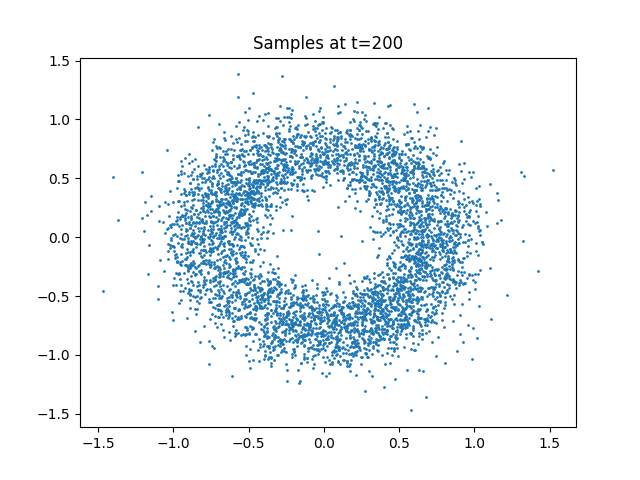
\includegraphics[width=0.3\textwidth]{exps/ddpm_2_200_0.0001_0.02_circles/samples_200.png} &
            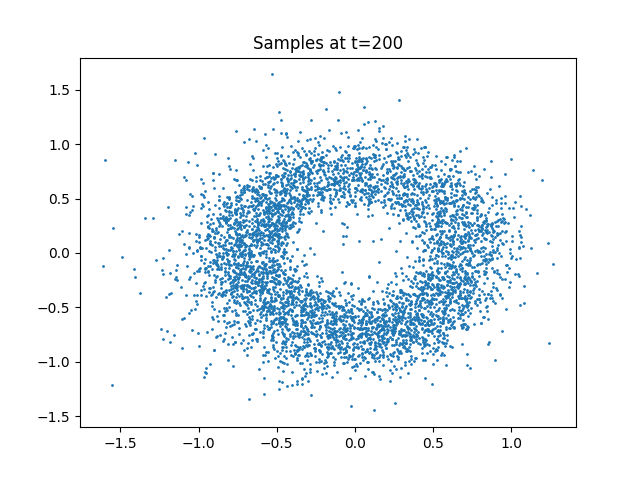
\includegraphics[width=0.3\textwidth]{exps/ddpm_2_200_0.001_0.2_circles/samples_200.png} &
            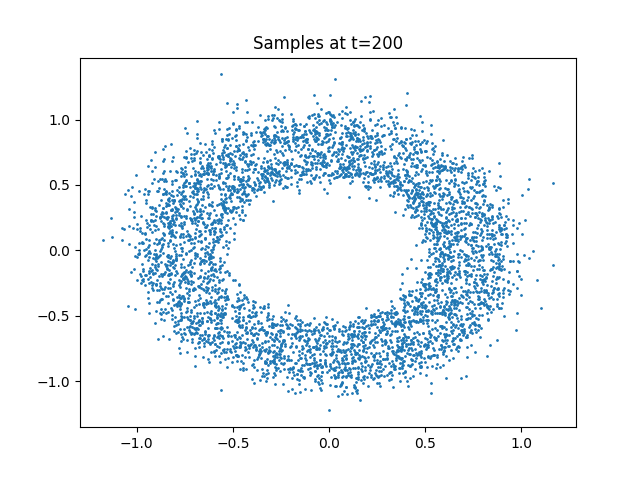
\includegraphics[width=0.3\textwidth]{exps/ddpm_2_200_1e-05_0.002_circles/samples_200.png} \\
            $\beta=1\text{e-}4\to0.02$ & $\beta=1\text{e-}3\to0.2$ & $\beta=1\text{e-}5\to0.002$ \\[0.5em]
            
            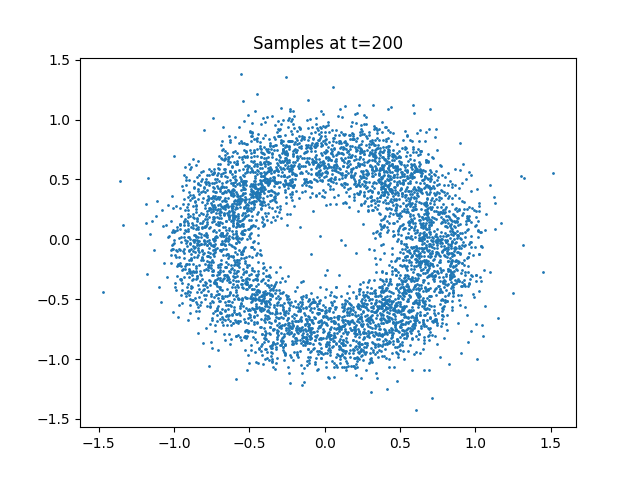
\includegraphics[width=0.3\textwidth]{exps/ddpm_2_200_1e-05_0.02_circles/samples_200.png} &
            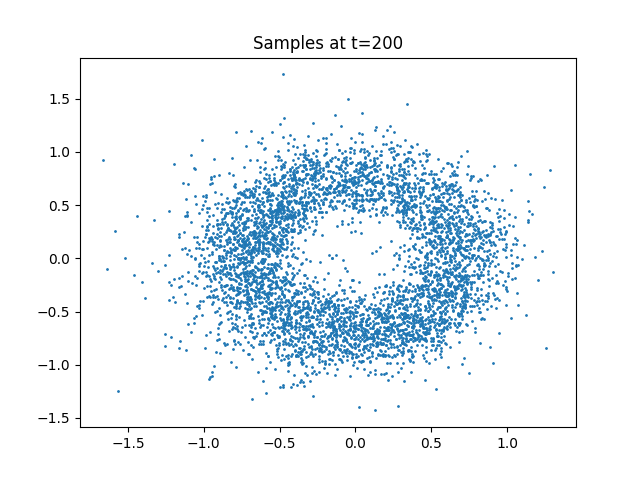
\includegraphics[width=0.3\textwidth]{exps/ddpm_2_200_0.0001_0.2_circles/samples_200.png} &
            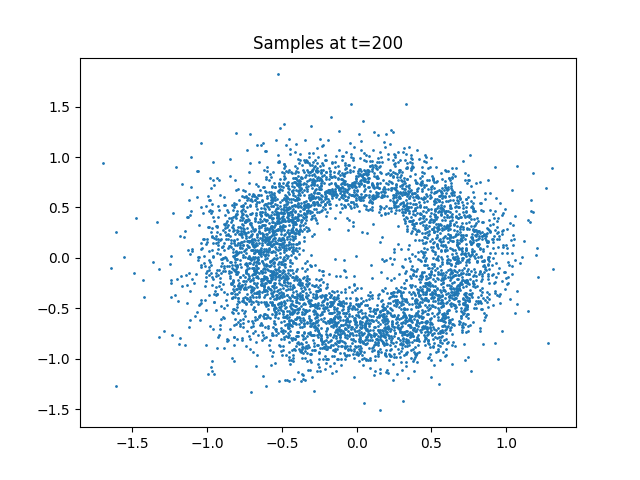
\includegraphics[width=0.3\textwidth]{exps/ddpm_2_200_1e-05_0.2_circles/samples_200.png} \\
            $\beta=1\text{e-}5\to0.02$ & $\beta=1\text{e-}4\to0.2$ & $\beta=1\text{e-}5\to0.2$ \\
        \end{tabular}
        \caption{Samples generated by DDPM with \textbf{varying beta schedules} for the Circles dataset.}
        \label{fig:beta_circles}
    \end{figure}

    \begin{figure}[H]
        \centering
        \begin{tabular}{ccc}
            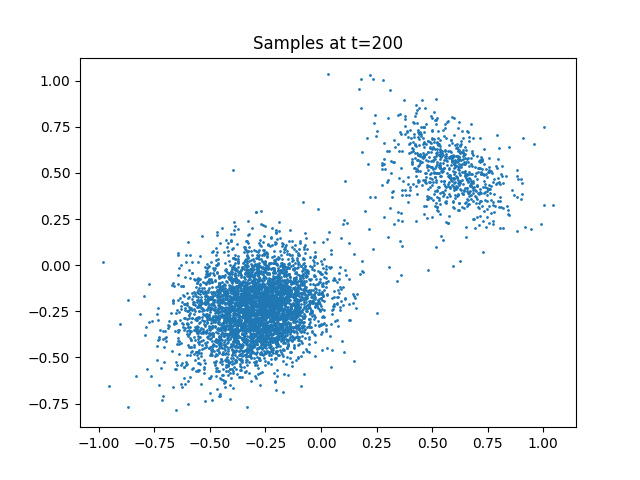
\includegraphics[width=0.3\textwidth]{exps/ddpm_2_200_0.0001_0.02_blobs/samples_200.png} &
            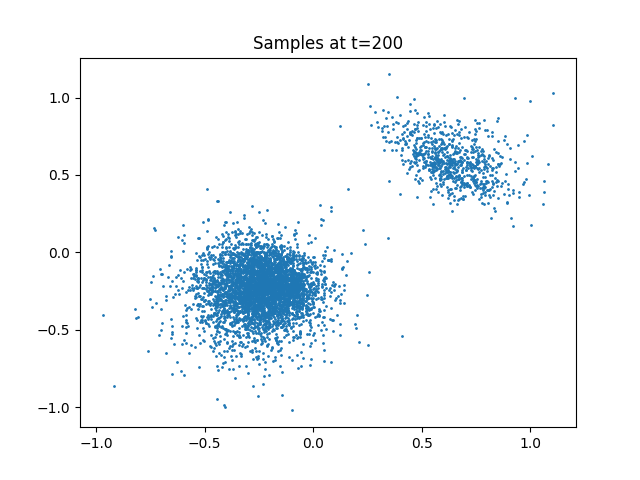
\includegraphics[width=0.3\textwidth]{exps/ddpm_2_200_0.001_0.2_blobs/samples_200.png} &
            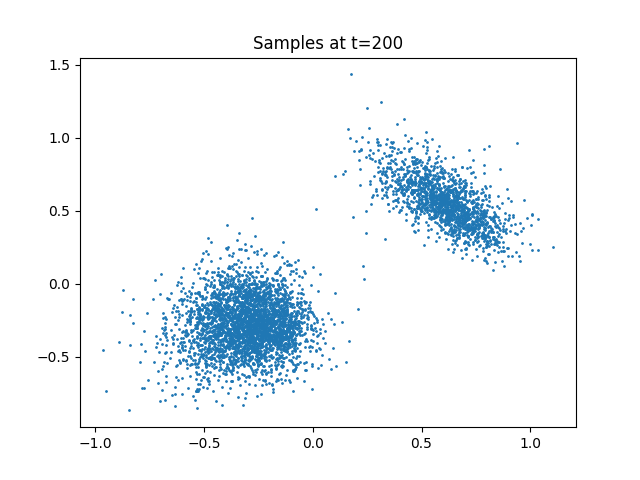
\includegraphics[width=0.3\textwidth]{exps/ddpm_2_200_1e-05_0.002_blobs/samples_200.png} \\
            $\beta=1\text{e-}4\to0.02$ & $\beta=1\text{e-}3\to0.2$ & $\beta=1\text{e-}5\to0.002$ \\[0.5em]
            
            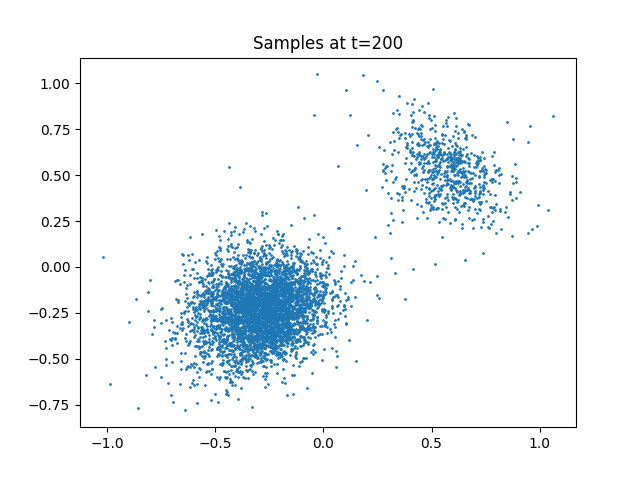
\includegraphics[width=0.3\textwidth]{exps/ddpm_2_200_1e-05_0.02_blobs/samples_200.png} &
            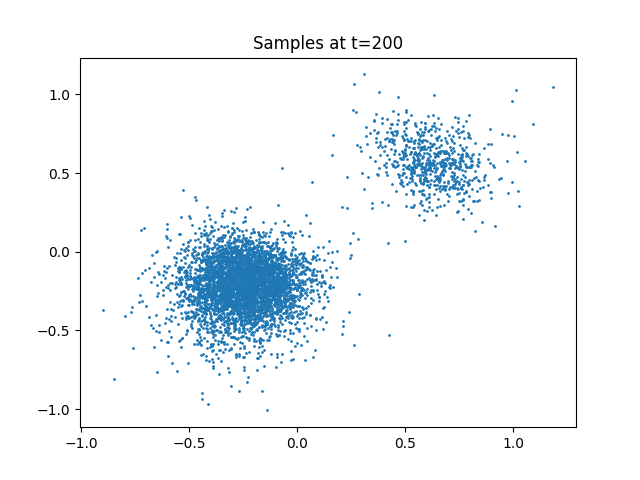
\includegraphics[width=0.3\textwidth]{exps/ddpm_2_200_0.0001_0.2_blobs/samples_200.png} &
            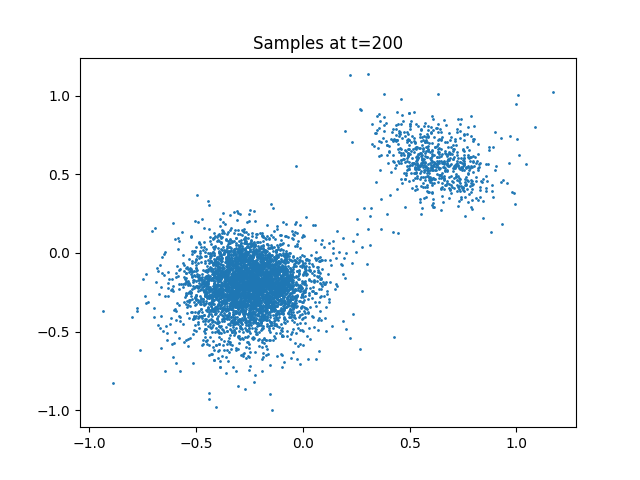
\includegraphics[width=0.3\textwidth]{exps/ddpm_2_200_1e-05_0.2_blobs/samples_200.png} \\
            $\beta=1\text{e-}5\to0.02$ & $\beta=1\text{e-}4\to0.2$ & $\beta=1\text{e-}5\to0.2$ \\
        \end{tabular}
        \caption{Samples generated by DDPM with \textbf{varying beta schedules} for the Blobs dataset.}
        \label{fig:beta_blobs}
    \end{figure}

    \begin{figure}[H]
        \centering
        \begin{tabular}{ccc}
            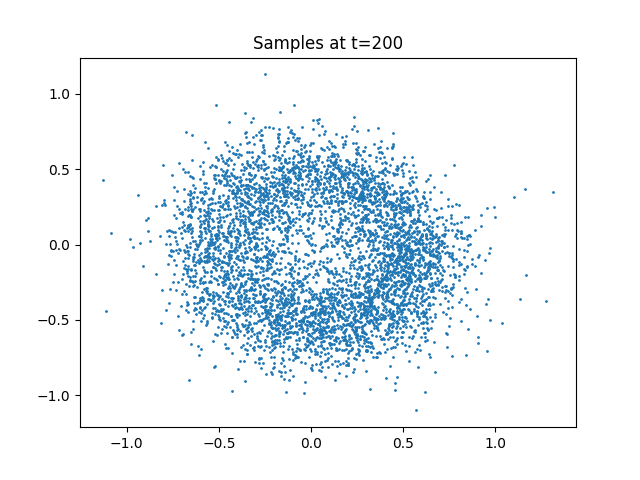
\includegraphics[width=0.3\textwidth]{exps/ddpm_2_200_0.0001_0.02_manycircles/samples_200.png} &
            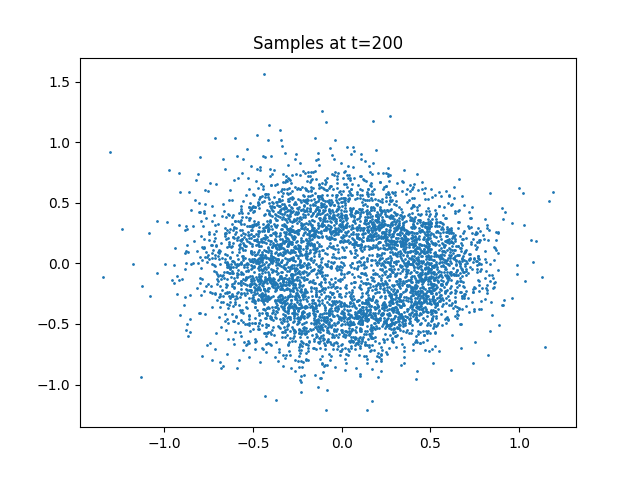
\includegraphics[width=0.3\textwidth]{exps/ddpm_2_200_0.001_0.2_manycircles/samples_200.png} &
            \includegraphics[width=0.3\textwidth]{exps/ddpm_2_200_1e-05_0.002_manycircles/samples_200.png} \\
            $\beta=1\text{e-}4\to0.02$ & $\beta=1\text{e-}3\to0.2$ & $\beta=1\text{e-}5\to0.002$ \\[0.5em]
            
            \includegraphics[width=0.3\textwidth]{exps/ddpm_2_200_1e-05_0.02_manycircles/samples_200.png} &
            \includegraphics[width=0.3\textwidth]{exps/ddpm_2_200_0.0001_0.2_manycircles/samples_200.png} &
            \includegraphics[width=0.3\textwidth]{exps/ddpm_2_200_1e-05_0.2_manycircles/samples_200.png} \\
            $\beta=1\text{e-}5\to0.02$ & $\beta=1\text{e-}4\to0.2$ & $\beta=1\text{e-}5\to0.2$ \\
        \end{tabular}
        \caption{Samples generated by DDPM with \textbf{varying beta schedules} for the Manycircles dataset.}
        \label{fig:beta_manycircles}
    \end{figure}

    \begin{figure}[H]
        \centering
        \begin{tabular}{ccc}
            \includegraphics[width=0.3\textwidth]{exps/ddpm_3_200_0.0001_0.02_helix/samples_200.png} &
            \includegraphics[width=0.3\textwidth]{exps/ddpm_3_200_0.001_0.2_helix/samples_200.png} &
            \includegraphics[width=0.3\textwidth]{exps/ddpm_3_200_1e-05_0.002_helix/samples_200.png} \\
            $\beta=1\text{e-}4\to0.02$ & $\beta=1\text{e-}3\to0.2$ & $\beta=1\text{e-}5\to0.002$ \\[0.5em]
            
            \includegraphics[width=0.3\textwidth]{exps/ddpm_3_200_1e-05_0.02_helix/samples_200.png} &
            \includegraphics[width=0.3\textwidth]{exps/ddpm_3_200_0.0001_0.2_helix/samples_200.png} &
            \includegraphics[width=0.3\textwidth]{exps/ddpm_3_200_1e-05_0.2_helix/samples_200.png} \\
            $\beta=1\text{e-}5\to0.02$ & $\beta=1\text{e-}4\to0.2$ & $\beta=1\text{e-}5\to0.2$ \\
        \end{tabular}
        \caption{Samples generated by DDPM with \textbf{varying beta schedules} for the Helix dataset.}
        \label{fig:beta_helix}
    \end{figure}

\subsubsection{Training Albatross}
The hyperparameters used for training Albatross are as follows:
\begin{itemize}
    \item \textbf{Timesteps}: 150
    \item \textbf{Beta Schedule}: 1e-4→0.02
\end{itemize}

\section{Classifier-Free Guidance}

For EMD calculation, the number of subsamples is set to 250 and the number of iterations is set to 5.

For all training runs, the hyperparameters used are as follows:
\begin{itemize}
    \item \textbf{Epochs}: 100
    \item \textbf{Batch Size}: 64
    \item \textbf{Learning Rate}: 1e-3
    \item \textbf{lbeta}: 0.0001
    \item \textbf{ubeta}: 0.02
    \item \textbf{p\_uncond} (required for CFG training): 0.2
\end{itemize}

\subsection{Guided vs. Conditional Sampling}

\begin{itemize}
    \item \textbf{Training:} Conditional sampling requires the model to be trained with explicit labels, while guided sampling can work even with an unconditional model.
    
    \item \textbf{Control:} Conditional sampling directly conditions the model on labels, whereas guided sampling modifies the noise prediction using a guidance scale.
    
    \item \textbf{Flexibility:} Conditional sampling is fixed after training, while guided sampling allows dynamic tuning of the guidance strength during inference.
    
    \item \textbf{Diversity:} Conditional sampling maintains diversity in generated samples, but guided sampling can reduce diversity if the guidance scale is too high.
    
    \item \textbf{Best Use Case:} Conditional sampling is ideal when training a model from scratch, while guided sampling is useful when modifying an already trained model.
\end{itemize}

\subsection{Architecture}

The model architecture for Classifier-Free Guidance (CFG) is similar to DDPM, with the modification of concatenating a class embedding to the input layer. The class embedding is a sinusoidal position embedding similar to the time embedding used in DDPM.

\subsection{Conditional DDPM Results}

\begin{figure}[H]
    \centering
    \begin{tabular}{ccc}
        \includegraphics[width=0.3\textwidth]{exps/ddpm_2_150_0.0001_0.02_moons/samples_conditional_150.png} &
        \includegraphics[width=0.3\textwidth]{exps/ddpm_2_150_0.0001_0.02_circles/samples_conditional_150.png} &
        \includegraphics[width=0.3\textwidth]{exps/ddpm_2_150_0.0001_0.02_manycircles/samples_conditional_150.png} \\
        Moons & Circles & Manycircles \\[0.5em]

        
        \includegraphics[width=0.3\textwidth]{exps/ddpm_2_150_0.0001_0.02_blobs/samples_conditional_150.png} &
        \includegraphics[width=0.3\textwidth]{exps/ddpm_3_150_0.0001_0.02_helix/samples_conditional_150.png} & \\
        Blobs & Helix & \\
    \end{tabular}
    \caption{Samples generated by \textbf{conditional} DDPM for various datasets.}
    \label{fig:cond_all_data}
\end{figure}

\subsection{Classifier-Free Guidance Results}

\begin{longtable}{|l|l|c|c|c|c|c|}
    \hline
    \textbf{Dataset} & \textbf{Metric} & \multicolumn{5}{c|}{\textbf{Guidance Scale}} \\
    \cline{3-7}
    & & \textbf{0.25} & \textbf{0.5} & \textbf{1.0} & \textbf{2.0} & \textbf{4.0} \\
    \hline
    \multirow{2}{*}{Moons} & EMD & \textbf{27.23} & 31.77 & 44.57 & 63.59 & 82.62 \\
    \cline{2-7}
    & Accuracy & \textbf{1.00} & \textbf{1.00} & \textbf{1.00} & \textbf{1.00} & \textbf{1.00} \\
    \hline
    \multirow{2}{*}{Circles} & EMD & 40.60 & \textbf{40.33} & 40.65 & 42.87 & 56.30 \\
    \cline{2-7}
    & Accuracy & 0.97 & 0.99 & \textbf{1.00} & \textbf{1.00} & \textbf{1.00} \\
    \hline
    \multirow{2}{*}{Blobs} & EMD & \textbf{20.27} & 26.16 & 39.27 & 55.48 & 77.69 \\
    \cline{2-7}
    & Accuracy & 0.95 & 0.98 & 0.99 & \textbf{1.00} & \textbf{1.00} \\
    \hline
    \multirow{2}{*}{Manycircles} & EMD & \textbf{12.16} & 14.62 & 18.97 & 25.14 & 34.04 \\
    \cline{2-7}
    & Accuracy & 0.92 & 0.96 & 0.98 & \textbf{1.00} & \textbf{1.00} \\
    \hline
    \multirow{2}{*}{Helix} & EMD & \textbf{56.82} & 58.13 & 63.17 & 74.67 & 97.19 \\
    \cline{2-7}
    & Accuracy & 0.73 & 0.76 & 0.82 & 0.88 & \textbf{0.94} \\
    \hline
\end{longtable}
\label{tab:cfg_results}

We observe a clear trade-off between sample quality (measured by EMD) and conditional accuracy across all datasets. As the guidance scale increases, the accuracy generally improves. However, this comes at the cost of increasing EMD values, suggesting that the generated samples may stray further from the true data distribution.

\begin{figure}[H]
    \centering
    \begin{tabular}{ccc}
        \includegraphics[width=0.3\textwidth]{exps/ddpm_2_150_0.0001_0.02_moons/samples_cfg_150_0.25.png} &
        \includegraphics[width=0.3\textwidth]{exps/ddpm_2_150_0.0001_0.02_moons/samples_cfg_150_0.5.png} &
        \includegraphics[width=0.3\textwidth]{exps/ddpm_2_150_0.0001_0.02_moons/samples_cfg_150_1.0.png} \\
        guidance=0.25 & guidance=0.5 & guidance=1.0 \\ [0.5em]

        \includegraphics[width=0.3\textwidth]{exps/ddpm_2_150_0.0001_0.02_moons/samples_cfg_150_2.0.png} &
        \includegraphics[width=0.3\textwidth]{exps/ddpm_2_150_0.0001_0.02_moons/samples_cfg_150_4.0.png} & \\
        guidance=2.0 & guidance=4.0 & \\
    \end{tabular}
    \caption{Samples generated by DDPM with \textbf{varying guidance scales} for the Moons dataset.}
    \label{fig:guidance_moons}
\end{figure}

\begin{figure}[H]
    \centering
    \begin{tabular}{ccc}
        \includegraphics[width=0.3\textwidth]{exps/ddpm_2_150_0.0001_0.02_circles/samples_cfg_150_0.25.png} &
        \includegraphics[width=0.3\textwidth]{exps/ddpm_2_150_0.0001_0.02_circles/samples_cfg_150_0.5.png} &
        \includegraphics[width=0.3\textwidth]{exps/ddpm_2_150_0.0001_0.02_circles/samples_cfg_150_1.0.png} \\
        guidance=0.25 & guidance=0.5 & guidance=1.0 \\ [0.5em]

        \includegraphics[width=0.3\textwidth]{exps/ddpm_2_150_0.0001_0.02_circles/samples_cfg_150_2.0.png} &
        \includegraphics[width=0.3\textwidth]{exps/ddpm_2_150_0.0001_0.02_circles/samples_cfg_150_4.0.png} & \\
        guidance=2.0 & guidance=4.0 & \\
    \end{tabular}
    \caption{Samples generated by DDPM with \textbf{varying guidance scales} for the Circles dataset.}
    \label{fig:guidance_circles}
\end{figure}

\begin{figure}[H]
    \centering
    \begin{tabular}{ccc}
        \includegraphics[width=0.3\textwidth]{exps/ddpm_2_150_0.0001_0.02_blobs/samples_cfg_150_0.25.png} &
        \includegraphics[width=0.3\textwidth]{exps/ddpm_2_150_0.0001_0.02_blobs/samples_cfg_150_0.5.png} &
        \includegraphics[width=0.3\textwidth]{exps/ddpm_2_150_0.0001_0.02_blobs/samples_cfg_150_1.0.png} \\
        guidance=0.25 & guidance=0.5 & guidance=1.0 \\ [0.5em]

        \includegraphics[width=0.3\textwidth]{exps/ddpm_2_150_0.0001_0.02_blobs/samples_cfg_150_2.0.png} &
        \includegraphics[width=0.3\textwidth]{exps/ddpm_2_150_0.0001_0.02_blobs/samples_cfg_150_4.0.png} & \\
        guidance=2.0 & guidance=4.0 & \\
    \end{tabular}
    \caption{Samples generated by DDPM with \textbf{varying guidance scales} for the Blobs dataset.}
    \label{fig:guidance_blobs}
\end{figure}

\begin{figure}[H]
    \centering
    \begin{tabular}{ccc}
        \includegraphics[width=0.3\textwidth]{exps/ddpm_2_150_0.0001_0.02_manycircles/samples_cfg_150_0.25.png} &
        \includegraphics[width=0.3\textwidth]{exps/ddpm_2_150_0.0001_0.02_manycircles/samples_cfg_150_0.5.png} &
        \includegraphics[width=0.3\textwidth]{exps/ddpm_2_150_0.0001_0.02_manycircles/samples_cfg_150_1.0.png} \\
        guidance=0.25 & guidance=0.5 & guidance=1.0 \\ [0.5em]

        \includegraphics[width=0.3\textwidth]{exps/ddpm_2_150_0.0001_0.02_manycircles/samples_cfg_150_2.0.png} &
        \includegraphics[width=0.3\textwidth]{exps/ddpm_2_150_0.0001_0.02_manycircles/samples_cfg_150_4.0.png} & \\
        guidance=2.0 & guidance=4.0 & \\
    \end{tabular}
    \caption{Samples generated by DDPM with \textbf{varying guidance scales} for the Manycircles dataset.}
    \label{fig:guidance_manycircles}
\end{figure}

\begin{figure}[H]
    \centering
    \begin{tabular}{ccc}
        \includegraphics[width=0.3\textwidth]{exps/ddpm_3_150_0.0001_0.02_helix/samples_cfg_150_0.25.png} &
        \includegraphics[width=0.3\textwidth]{exps/ddpm_3_150_0.0001_0.02_helix/samples_cfg_150_0.5.png} &
        \includegraphics[width=0.3\textwidth]{exps/ddpm_3_150_0.0001_0.02_helix/samples_cfg_150_1.0.png} \\
        guidance=0.25 & guidance=0.5 & guidance=1.0 \\ [0.5em]
        
        \includegraphics[width=0.3\textwidth]{exps/ddpm_3_150_0.0001_0.02_helix/samples_cfg_150_2.0.png} &
        \includegraphics[width=0.3\textwidth]{exps/ddpm_3_150_0.0001_0.02_helix/samples_cfg_150_4.0.png} & \\
        guidance=2.0 & guidance=4.0 & \\
    \end{tabular}
    \caption{Samples generated by DDPM with \textbf{varying guidance scales} for the Helix dataset.}
    \label{fig:guidance_helix}
\end{figure}



% \section*{Acknowledgements}



\end{document}